\documentclass[../Main.tex]{subfiles}

\definecolor{codegreen}{rgb}{0,0.6,0}
\definecolor{codegray}{rgb}{0.5,0.5,0.5}
\definecolor{codepurple}{rgb}{0.58,0,0.82}
\definecolor{backcolour}{rgb}{0.95,0.95,0.92}

\lstdefinestyle{mystyle}{
    backgroundcolor=\color{backcolour},   
    commentstyle=\color{codegreen},
    keywordstyle=\color{magenta},
    numberstyle=\tiny\color{codegray},
    stringstyle=\color{codepurple},
    basicstyle=\ttfamily\footnotesize,
    breakatwhitespace=false,         
    breaklines=true,                 
    captionpos=b,                    
    keepspaces=true,                 
    numbers=left,                    
    numbersep=5pt,                  
    showspaces=false,                
    showstringspaces=false,
    showtabs=false,                  
    tabsize=2
}

\lstset{style=mystyle}
\begin{document}

    \section{Pruebas unitarias}
    \subsection{Descripción}
    \begin{justify}
    Las pruebas unitarias o unit testing lo que busca es corroborar el comportamiento correcto de una unidad de código.
    
    Django proporciona un framework de pruebas con una pequeña jerarquía de clases que se basan en la librería unittest estándar Python, esta librería es adecuada tanto para pruebas unitarias como pruebas de integración, en el backend del prototipo web GQuestions se hicieron pruebas unitarias.  
    
    Django ofrece métodos y herramientas que ayudan a probar el comportamiento, estos permiten simular las solicitudes con inserción de datos de prueba e inspección de la respuesta a las solicitudes.
    
    Para escribir pruebas existen clases base de prueba de Django como SimpleTestCase, TransactionTestCase, TestCase, LiveServerTestCase. En el backend se realizaron pruebas utilizando la clase base \textbf{TestCase}, se escribieron métodos por separado para verificar que los modelos del proyecto que hacen parte del diseño propio no tuviesen errores.
    
    \subsection{Detalles}
    Se probó aspectos del código escrito respecto a los modelos (base de datos) y no de bibliotecas o funcionalidades proporcionadas por Python o Django. Estos aspectos fueron el texto utilizado para etiquetas (atributos), tamaños de campos asignados y valores por defecto asignados.
    
    A continuación, se presentas algunos casos de prueba y posteriormente la creación de estas pruebas en Django con TestCase.
    \end{justify}
    
    \begin{table}[H]
	\begin{Center}
		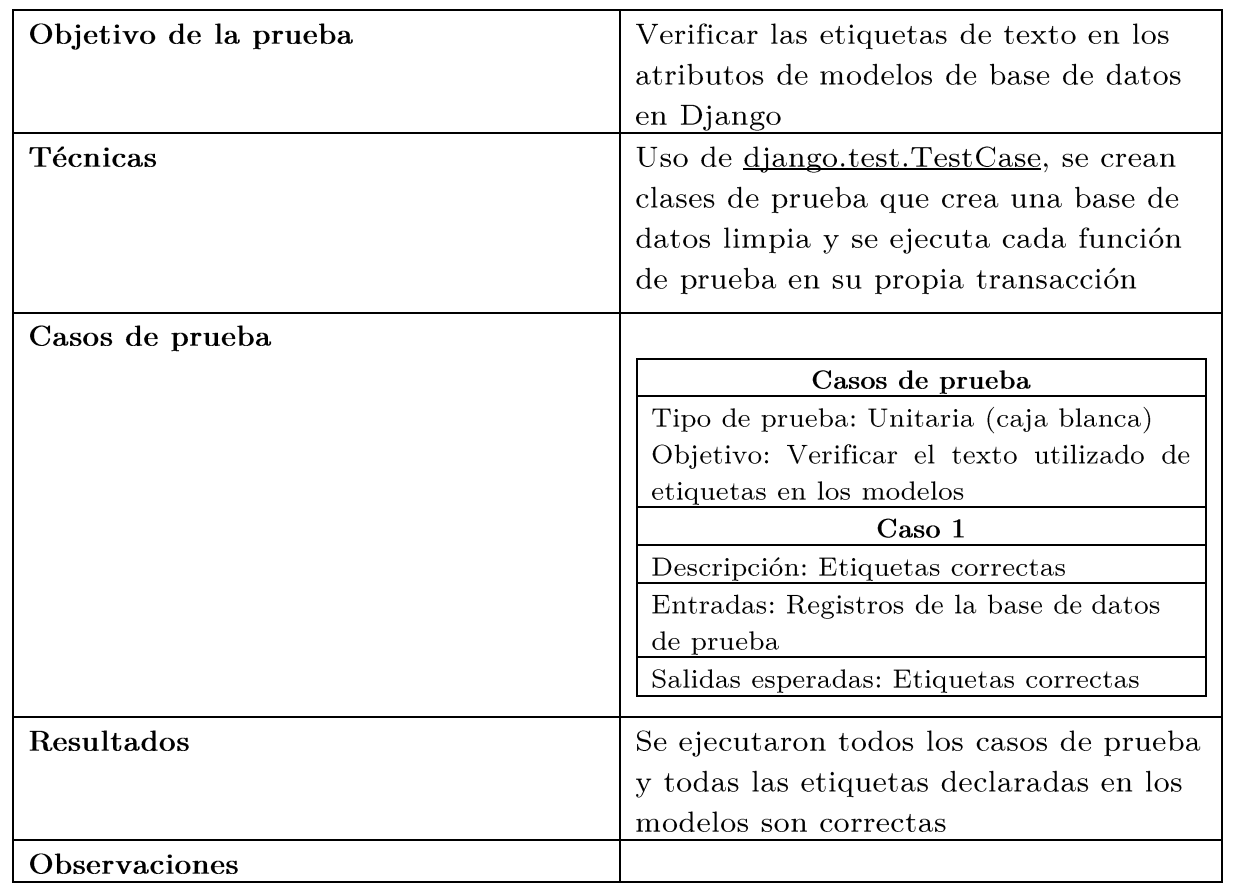
\includegraphics[width=5.8in,height=4.2in]{Chapters/06ChapterPruebas/images/caso_prueba_django.png}
	    \caption{Caso de prueba etiquetas de campos}
	    Fuente: Elaboración propia
        \label{tab:table1}
	\end{Center}
    \end{table}

       \begin{figure}[H]
	\begin{Center}
       \begin{lstlisting}[language=Python]
class GeneracionModel(models.Model):
    id = models.CharField(primary_key=True, null=False, max_length=255)
    n_examenes = models.SmallIntegerField(null=False)
    longit_texto = models.IntegerField(default=200)
    n_preguntas = models.SmallIntegerField(null=False)
    inicio_oracion = models.CharField(max_length=30, null=False, default='Aleatorio')
    fecha_generacion = models.DateTimeField(auto_now_add=True, null=False)
    account = models.ForeignKey(Account, related_name='account', on_delete=models.CASCADE)\end{lstlisting}
	    \caption{Modelo Generación - backend Django}
	    Fuente: Elaboración propia
        \label{fig:section}
	\end{Center}
    \end{figure}
    
    En la figura anterior se presenta el modelo Generación definido en Django, aquí se probó las etiquetas de todos los campos, porque a pesar de no haberse especificado explícitamente la mayoría se tiene un diseño que dice cuáles deben ser estos valores. Si no se prueban lo valores, entonces no se sabe que las etiquetas de los campos tienen efectivamente los valores deseados. De esta manera, sucede lo mismo con las longitudes de campo específicadas (max\_length) y valores por defecto (default).
    
    Para probar el modelo se comienza por crear una clase \texttt{GeneracionModelTest} que recibe como argumento \texttt{TestCase}. Se escribe un método de clase \texttt{setUpTestData} que permite la creación de datos de prueba iniciales.
    
    \begin{figure}[H]
	\begin{Center}
    \begin{lstlisting}[language=Python]
class GeneracionModelTest(TestCase):
@classmethod
def setUpTestData(cls):
    GeneracionModel.objects.create(
        id='ff6eb8f3-38a1', n_examenes=10, n_preguntas=5, account)\end{lstlisting}
    \caption{Clase Generación de prueba unitaria - backend Django}
	    Fuente: Elaboración propia
        \label{fig:section}
	\end{Center}
    \end{figure}
    
    Una vez se tiene el método de clase \texttt{setUpTestData} se escriben los métodos de clase de pruebas, como sigue:
    
    \begin{figure}[H]
	\begin{Center}
    \begin{lstlisting}[language=Python]
def test_n_examenes_label(self):
    gen=GeneracionModel.objects.get(id='ff6eb8f3-38a1')
    field_label = gen._meta.get_field('n_examenes').verbose_name
    self.assertEquals(field_label,'n examenes')\end{lstlisting}
        \caption{{Prueba unitaria etiqueta de campo - backend Django}}
	    Fuente: Elaboración propia
        \label{fig:section}
	\end{Center}
    \end{figure}
    
    En este caso se verifica que el campo tenga el valor de etiqueta de campo correcta \texttt{verbose\_name}, de manera similar se escribieron los pruebas de tamaño de campo y valores por defecto.
    
    \begin{figure}[H]
	\begin{Center}
    \begin{lstlisting}[language=Python]
def test_inicio_oracion_max_length(self):
    generacion=GeneracionModel.objects.get(id='ff6eb8f3-38a1')
    max_length = generacion._meta.get_field('inicio_oracion').max_length
    self.assertEquals(max_length, 30)\end{lstlisting}
        \caption{Prueba unitaria longitud de campo - backend Django}
	    Fuente: Elaboración propia
        \label{fig:section}
	\end{Center}
    \end{figure}
    
    \begin{figure}[H]
	\begin{Center}
    \begin{lstlisting}[language=Python]
def test_longit_text_default_value(self):
    generacion=GeneracionModel.objects.get(id='ff6eb8f3-38a1')
    default_value = generacion.longit_texto
    self.assertEquals(default_value, 200)\end{lstlisting}
        \caption{Prueba unitaria valor por defecto - backend Django}
	    Fuente: Elaboración propia
        \label{fig:section}
	\end{Center}
    \end{figure}
\end{document}

